\documentclass[12pt,letterpaper]{article}

\usepackage{amsmath, amsthm, amsfonts, amssymb}
\usepackage{graphicx,hyperref}
\usepackage{microtype, parskip}
\usepackage[comma,sort&compress]{natbib}
\usepackage{docmute}
\usepackage{subcaption, multirow, morefloats}
\usepackage{wrapfig, rotating}

\frenchspacing

\captionsetup[subfigure]{position = top, labelfont = bf, textfont = normalfont, singlelinecheck = off, justification = raggedright}

\begin{document}
\section{Methods}
\subsection{Species information}

\subsubsection{Informal phylogeny}

\subsection{Biogeographic network}

A biogeographic network is defined as a bipartite network between localities and taxa \citep{Vilhena2013b,Vilhena2013,Sidor2013}. The properties of a bipartite network are such that taxa are connected to localities, but taxa are not connected to taxa and localities are not connected to localities (Fig. \ref{subfig:bip_net}). In this study, taxa are defined as species and localities are defined as 2x2 latitude--longitude grid cells from an azimuthal equal-area map projection.

\begin{figure}[ht]
  \centering
  \begin{subfigure}[b]{0.4\textwidth}
    \caption{}
    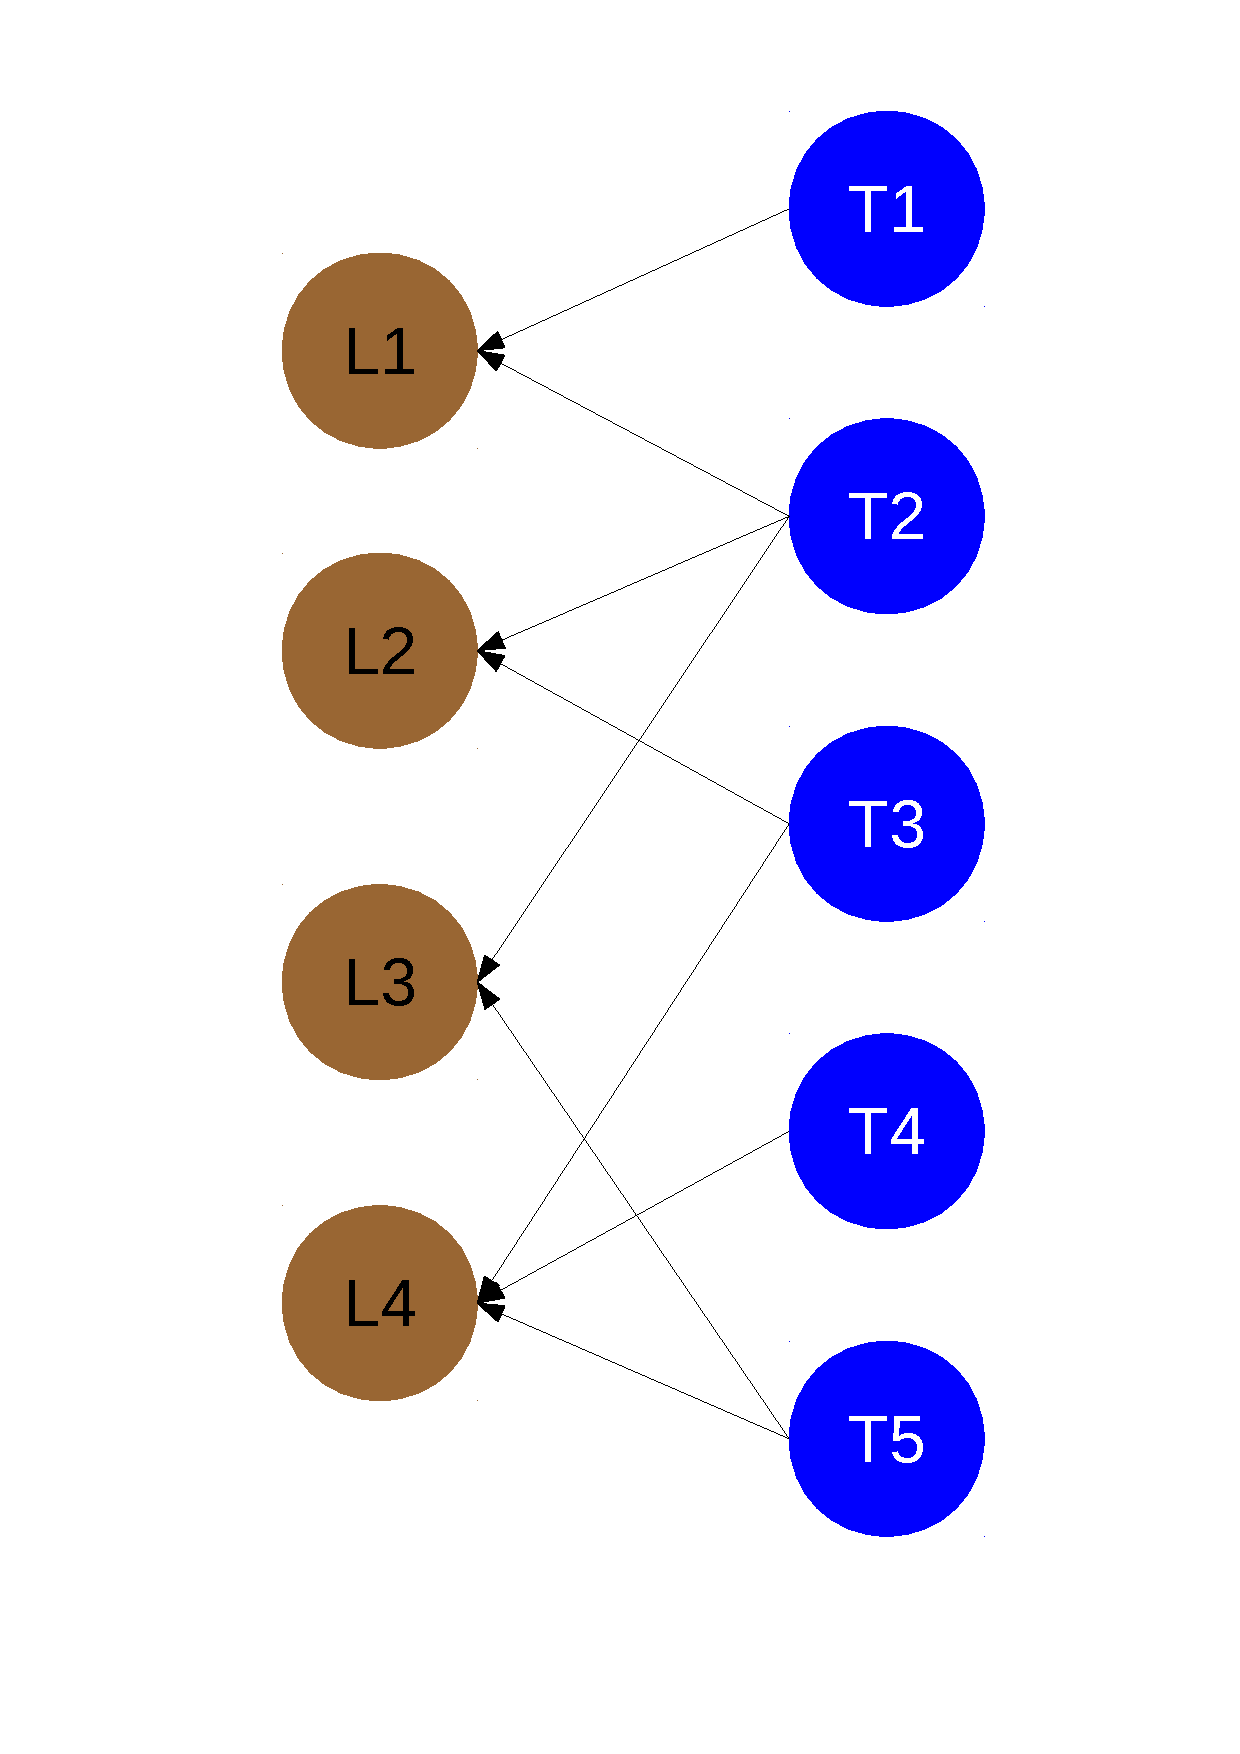
\includegraphics[height = 0.5\textheight, width = \textwidth, keepaspectratio = true]{figure/bipartite_graph}
    \label{subfig:bip_net}
  \end{subfigure}

  \begin{subfigure}[b]{0.4\textwidth}
    \caption{}
    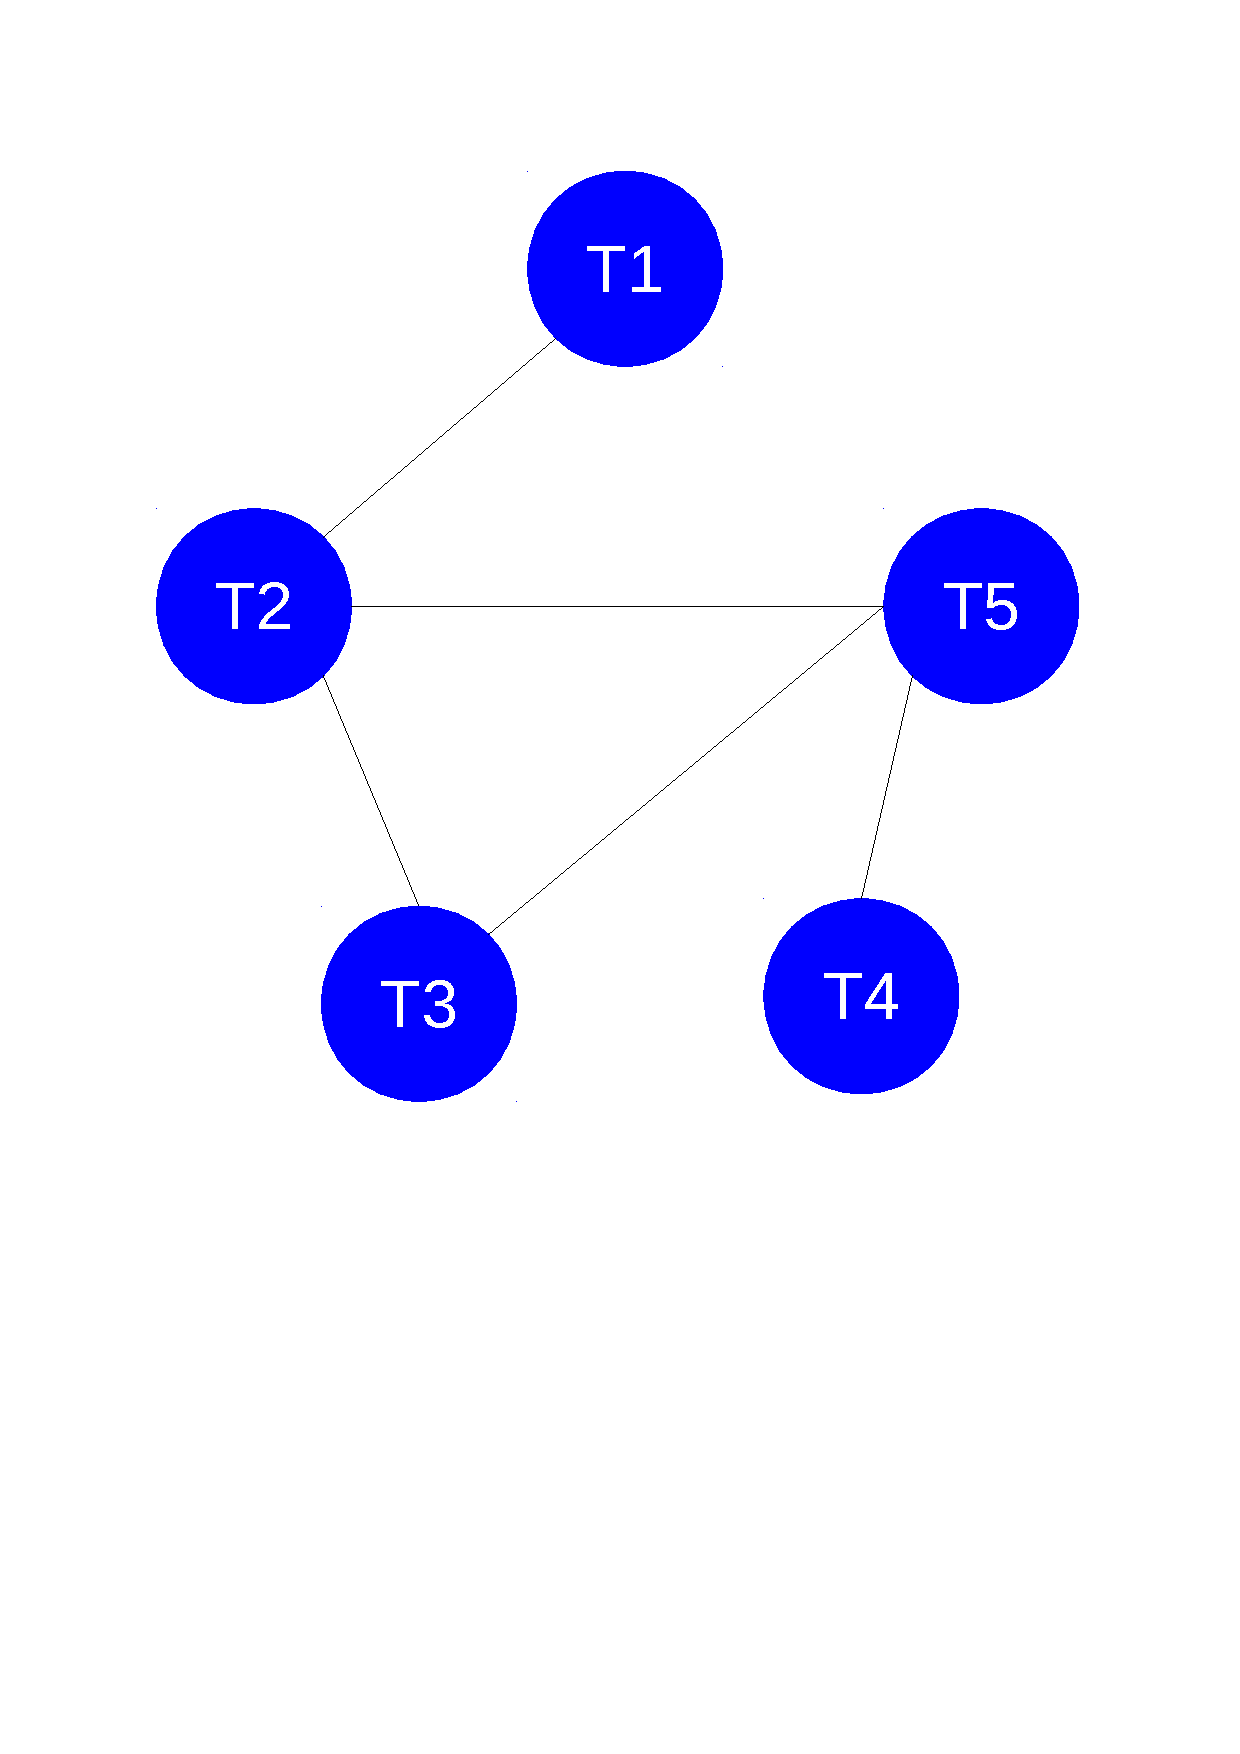
\includegraphics[height = 0.5\textheight, width = \textwidth, keepaspectratio = true]{figure/one_mode}
    \label{subfig:one_mode}
  \end{subfigure}
  \caption{Bipartite and one mode graphs.}
  \label{fig:graphs}
\end{figure}


\subsection{Co-occurrence model}
A random graph is one where the probability of any two nodes being connected is equal for all combinations \citep{Erdos1959}. This assumption implies that the distribution of nodal degree should follow a Poisson distribution. What this means is that the degree, or number of connections, of a node in a one mode network is considered drawn from a Poisson distribution with some rate, \(\lambda\).

The Poisson distribution with rate \(\lambda > 0\) is defined 
\begin{align}
  \mathrm{Poisson}(y_{i} | \lambda_{i}) &= \frac{1}{y_{i}!} \lambda^{y_{i}} \exp(-\lambda_{i}) 
  \label{eq:pois} \\
  \lambda_{i} &= \exp(\beta^{T}\mathbf{X_{i}} + h_{i} + \log(u_{i})).
  \label{eq:lambda}
\end{align}

The biggest assumption of the Poisson distribution is that mean and variance are equal is very strong and not frequently observed, instead there tends to be excess variance or overdisperssion. The negative binomial distribution can be viewed as an extension of the Poisson distribution allowing for overdispersion. 

Negative binomial distribution parameterized with mean \(\mu > 0\) and overdispersion \(\phi > 0\) is defined
\begin{align}
  \mathrm{Negative\ binomial}(y_{i} | \mu_{i}, \phi) &= {y_{i} + \phi -1 \choose y_{i}} \left(\frac{\mu_{i}}{\mu_{i} + \phi}\right)^{y_{i}} \left(\frac{\phi}{\mu_{i} + \phi}\right)^{\phi}
  \label{eq:neg_bin} \\
  \mu_{i} &= \exp(\beta^{T}\mathbf{X_{i}} + h_{i} + \log(u_{i})) 
  \label{eq:mu} \\
  \phi &\sim \mathrm{halfCauchy}(2.5).
  \label{eq:phi} 
\end{align}


\(\mathbf{X}\) is defined as an \(n \times K\) matrix where \(n\) is the number of observations and \(K\) is the number of covariates of interest. As described above, the covariates of interest are the dietary and locomotor categories of a species and its body mass. While body mass is a continuous covariate, dietary and locomotor categories are index variables that need to be transformed into multiple binary covariates or indicator variables. To do this, for each of these variables were each transformed into \(n \times (k - 1)\) matrices where \(k - 1\) is the number of categories of the index variable (3 and 4, respectively). Only \(k - 1\) indicator variables are necessary as the intercept takes on the remaining category. Finally, a column of 1-s in included in the matrix \(\mathbf{X}\) whose corresponding \(\beta\) coefficient is the intercept. In total, \(K\) equals 7.
% Do I want to change locomotor and dietary categories into random effects? Might improve interpretability.

For the parameterizations of the means for both the Poisson (Eq. \ref{eq:lambda}) and negative binomial models (Eq. \ref{eq:mu}), a unique coefficient \(\beta\) is assigned to each of the covariates and are given a diffuse, weakly informative prior (\(\beta_{k} \sim \mathcal{N}(0, 10)\)).

\(h\), or phylogenetic effect, is defined as a random multivariate normally distributed variable whose covariance matrix known up to a constant \(\sigma_{p}\) (Eq. \ref{eq:phy_sim}).
\begin{align}
  h &\sim \mathrm{Multivariate\ }\mathcal{N}(0, \mathbf{\Sigma}) \label{eq:phy_sim} \\
  \mathbf{\Sigma} &= \sigma_{p}^{2} \mathbf{V}_{phy} \nonumber \\
  \sigma_{p} &\sim \mathrm{halfCauchy}(2.5). \nonumber
\end{align}
This parameterization follows \citet{Lynch1991} and \citet{Housworth2004}.

\(u_{i}\) is the exposure term for observation \(i\) and is defined as the number of localities species \(i\) occurred in during the given stage. The inclusion of an exposure is so that the rate is more biologically interpretable as the rate is now in relation to some baseline. In this case, we can interpret \(\lambda\) as the expected number of co-occurring species per locality for a given observation. While \(u_{i}\) is called the exposure, \(\log(u_{i})\) is called the offset in the language generalized linear modeling \citep{Gelman2007}. The inclusion of \(\log(u_{i}\) in the parameterization of \(\mu_{i}\) is due to the following relationships 
\begin{align*}
  \mathrm{E}(Y) &= u_{i}\lambda_{i} \\
  \log(\mathrm{E}(Y)) &= \log(u_{i}) + \log(\lambda_{i}) \\
  \log(\mathrm{E}(Y)) &= \log(u_{i}) + \beta^{T}\mathbf{X_{i}} + h_{i} \\
  \log(\mathrm{E}(Y)) - \log(u_{i}) &= \beta^{T}\mathbf{X_{i}} + h_{i} \\
  \log\left(\frac{\mathrm{E}(Y)}{u_{i}}\right) &= \beta^{T}\mathbf{X_{i}} + h_{i}.
\end{align*}

The overdispersion parameter \(\phi\) of the negative binomial distribution was given weakly informative half-Cauchy prior distribution (Eq. \ref{eq:phi}).

Graphical summaries of the Poisson and negative binomial models, along with all values for the prior distributions, are presented in Figures \ref{fig:poismod_diagram} and \ref{fig:nbinmod_diagram}, respectively.
\begin{figure}[ht]
  \centering
  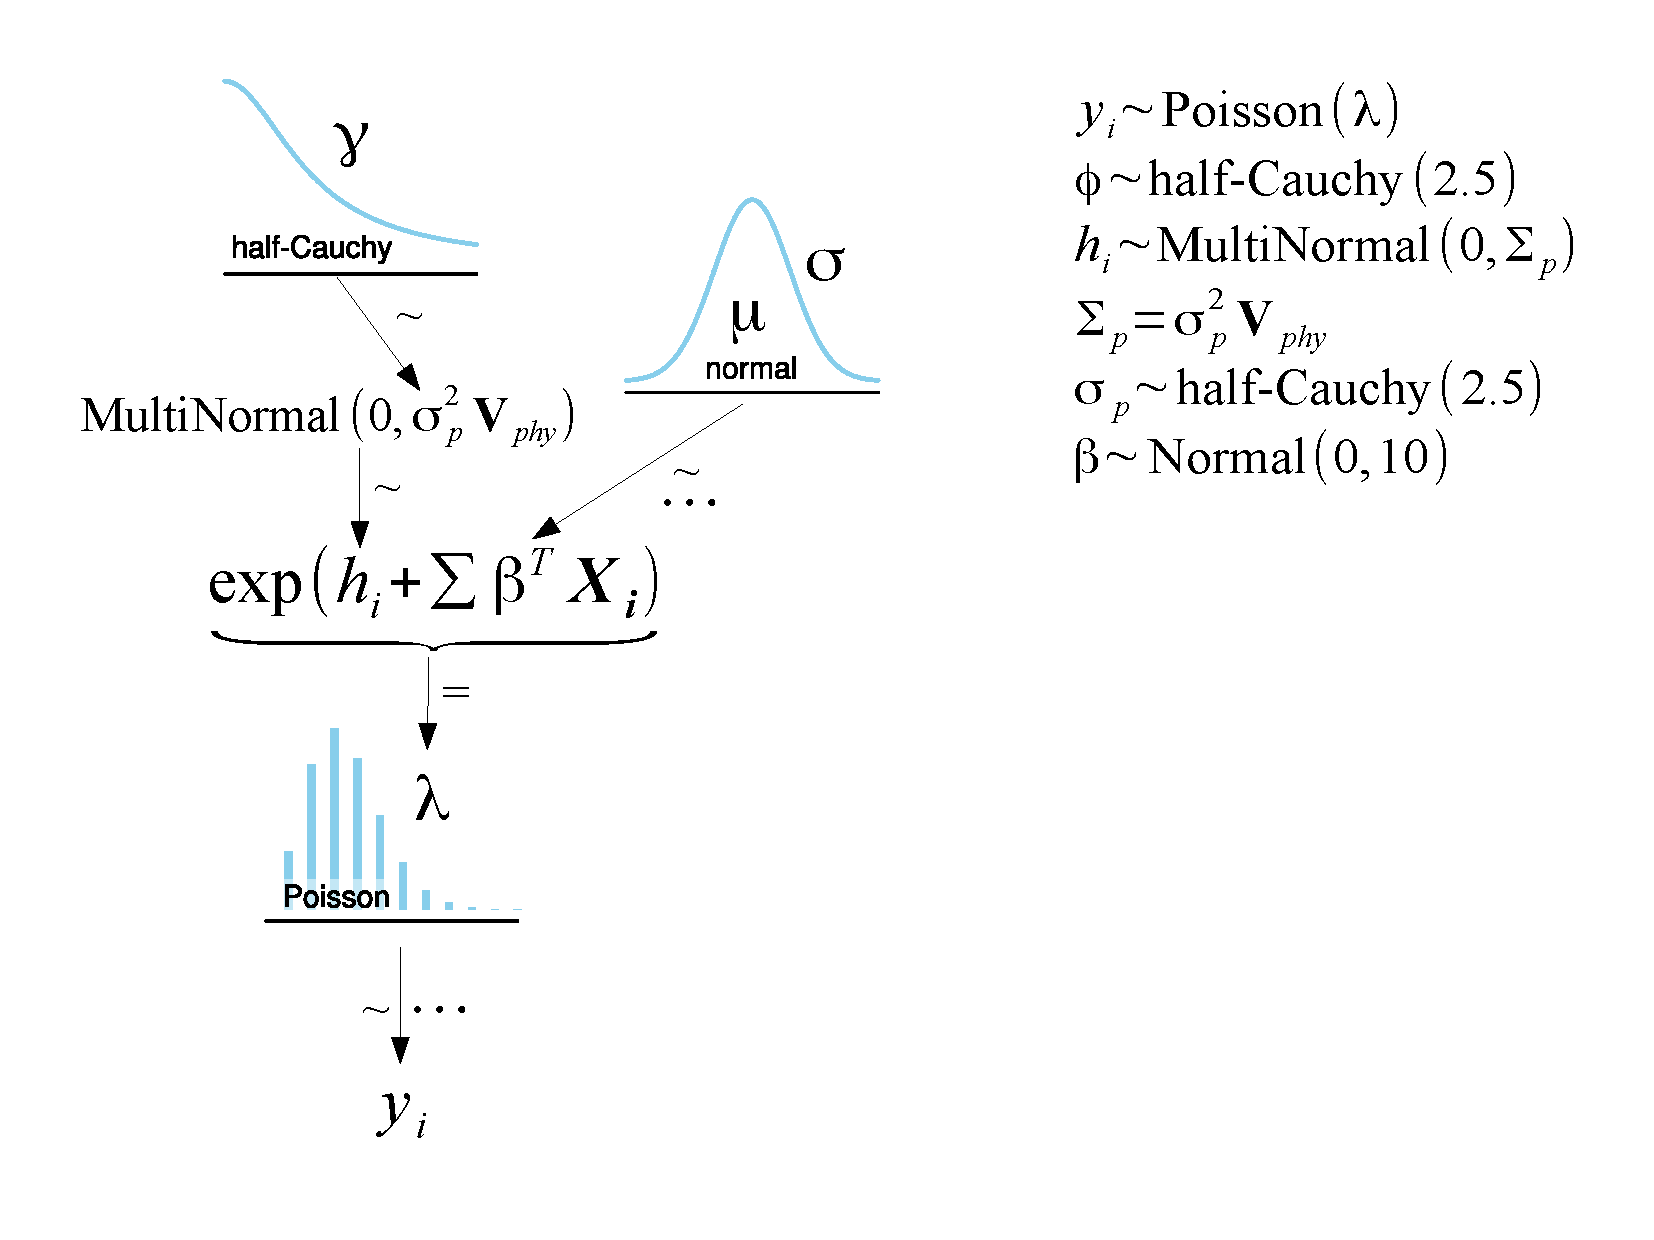
\includegraphics[height = 0.5\textheight, width = \textwidth, keepaspectratio = true]{figure/mammal_degree_model}
  \caption{Poisson model}
  \label{fig:poismod_diagram}
\end{figure}

\begin{figure}[ht]
  \centering
  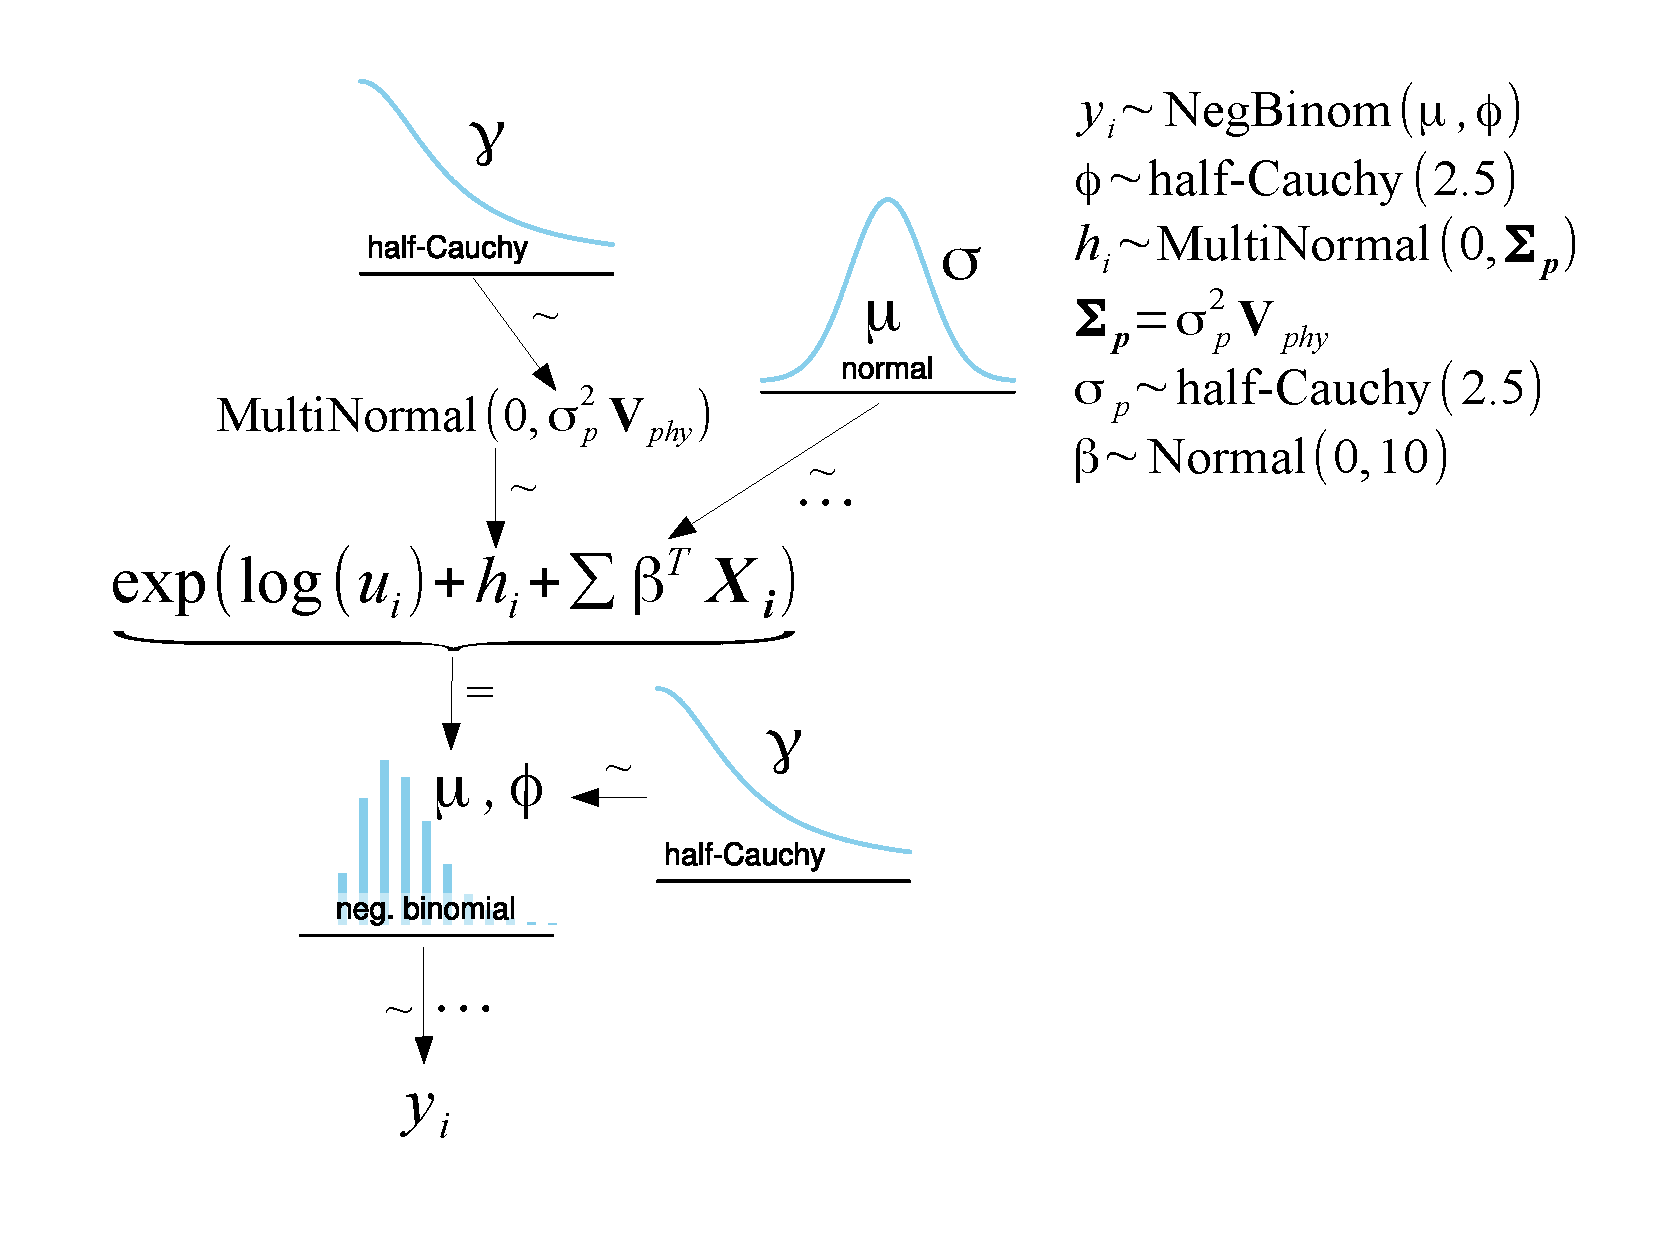
\includegraphics[height = 0.5\textheight, width = \textwidth, keepaspectratio = true]{figure/mammal_deg_over_model}
  \caption{Negative binomial model}
  \label{fig:nbinmod_diagram}
\end{figure}

\subsection{Posterior predictive checks}

A models utility in making predictive and descriptive statements is dependent on its fit to the data and the questions of interest. The most basic assessment of model fit is if, given known covariate information, values simulated from the model (\(y^{rep}\)) are similar to the observed (\(y\)). This is the idea behind posterior predictive checks \citep{Gelman2013d}. 

For all estimated parameters, a value is randomly drawn from their respective posteriors. These parameter estimates are then used with covariate information for all observations to make \(n\) estimates of the number of co-occurring species for a given species \(y^{rep}\). This process is repeated 1000 times to get a distribution of possible \(y^{rep}\)-s, which can then be compared to the original data \(y\) to assess the quality of model fit \citep{Gelman2013d}.


\subsection{Predictive estimates}

For each stage, 


\begin{figure}[ht]
  \centering
  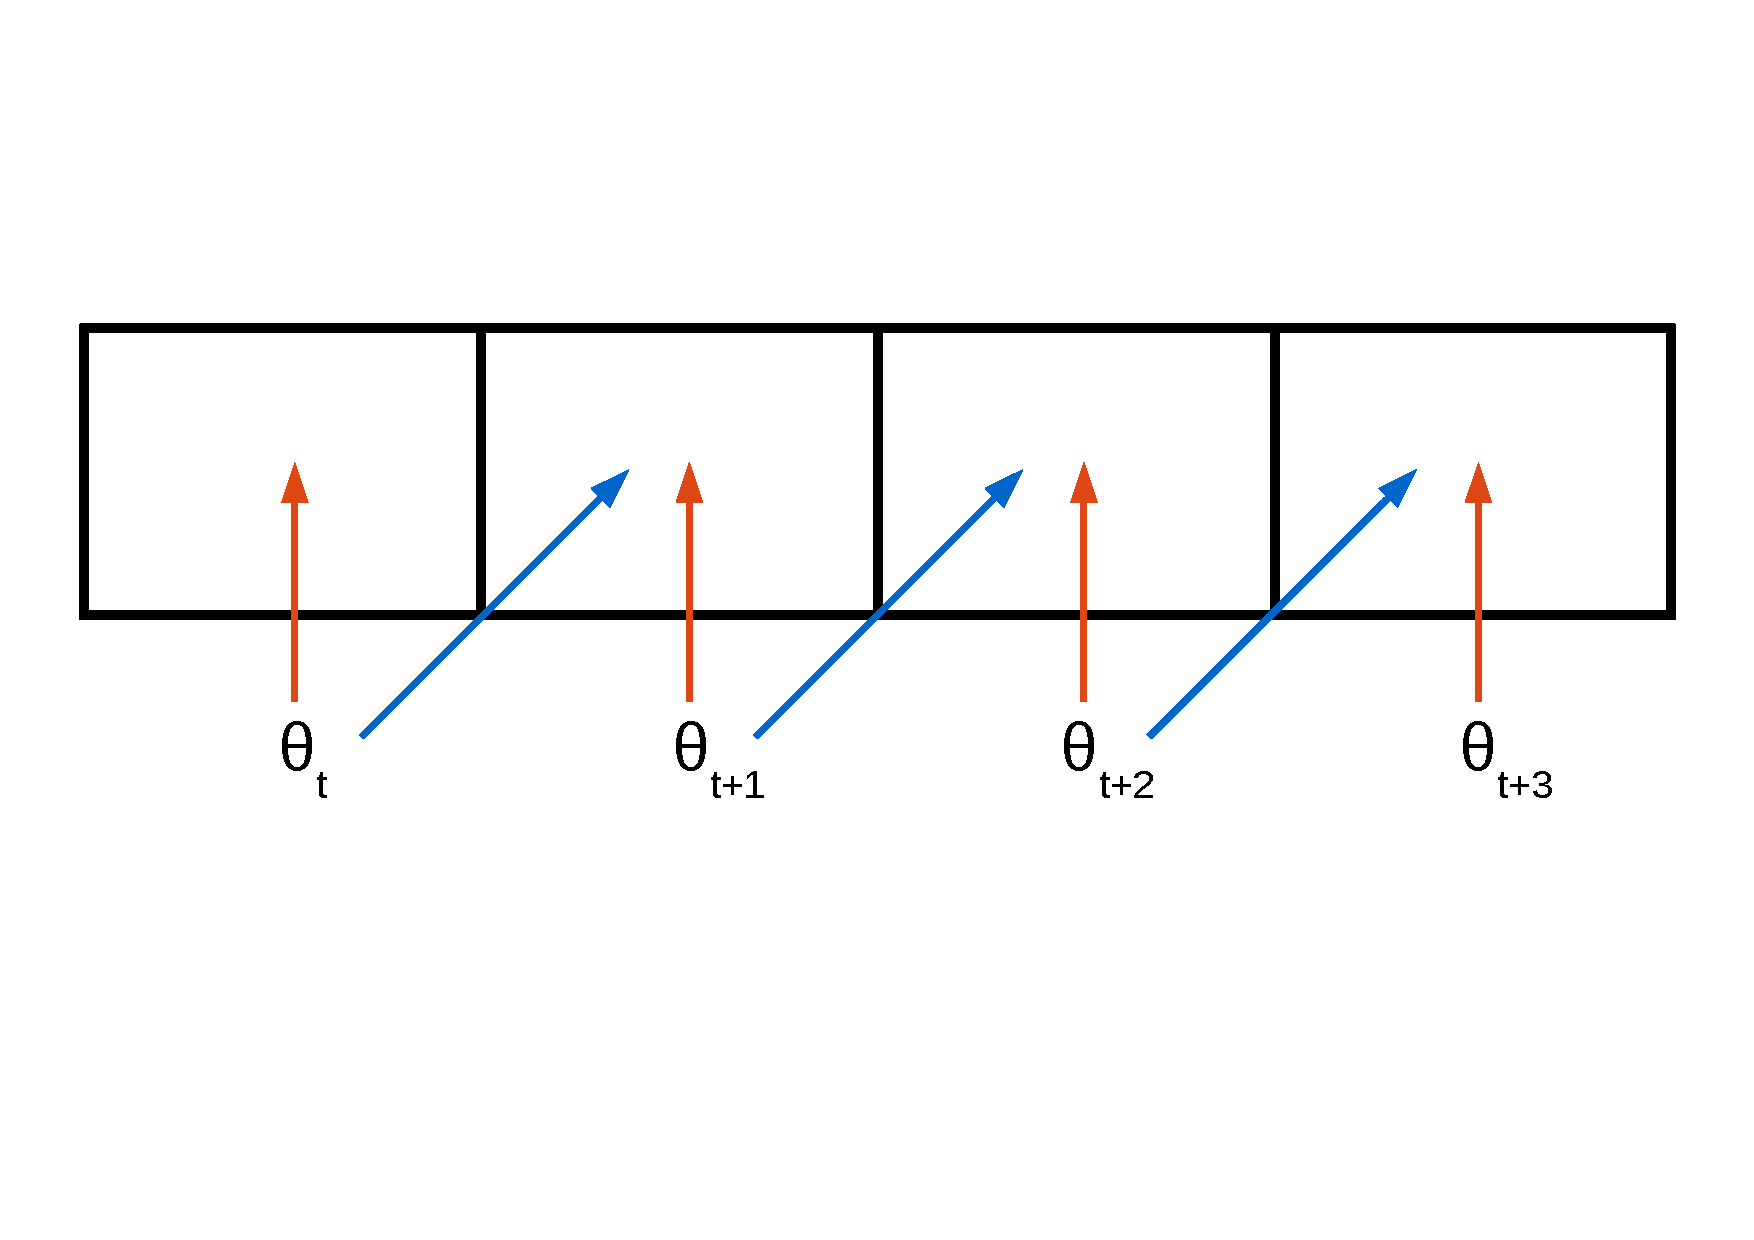
\includegraphics[height = 0.5\textheight, width = \textwidth, keepaspectratio = true]{figure/predict_perform}
  \caption{CAPTION}
  \label{fig:concept}
\end{figure}


\end{document}
